\begin{figure}[!h]
  \begin{center}
    \caption{Le segment $b$ cache une partie du segment $r$.}%
    \label{peintre:ill}
    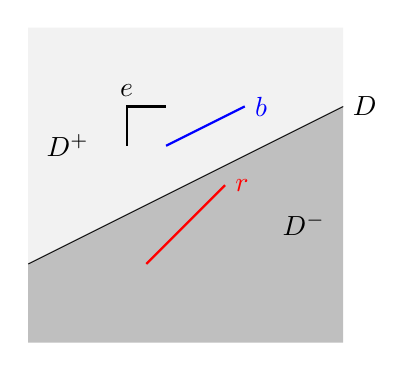
\begin{tikzpicture}
      \draw (-2, -1) -- (2, 1) node[right] {$D$};
      \fill [black, nearly transparent] %
      (-2, -1) -- (2, 1) -- (2, -2) -- (-2, -2) -- cycle;
      \draw (1.5, -0.5) node {$D^-$};
      \fill [black!20, nearly transparent] %
      (-2, -1) -- (2, 1) -- (2, 2) -- (-2, 2) -- cycle;
      \draw (-1.5, 0.5) node {$D^+$};
      \draw [thick](-0.75, 1) -- (-0.75, 0.5) -- (-0.75, 1)%
      node[above] {$e$} -- (-0.25, 1) ;
      \draw [blue, thick] (-0.25, 0.5) -- (0.75, 1) node[right] {$b$};
      \draw [red, thick] (-0.5, -1) -- (0.5, 0) node[right] {$r$};
    \end{tikzpicture}
\end{center}
\end{figure}

%%% Local Variables:
%%% mode: latex
%%% TeX-master: "../rapportGp1"
%%% End:
